\documentclass[border=0.2cm]{standalone}
 
% Bar chart drawing library 
\usepackage{pgfplots} 
\pgfplotsset{compat=1.18}
 
\begin{document}
 
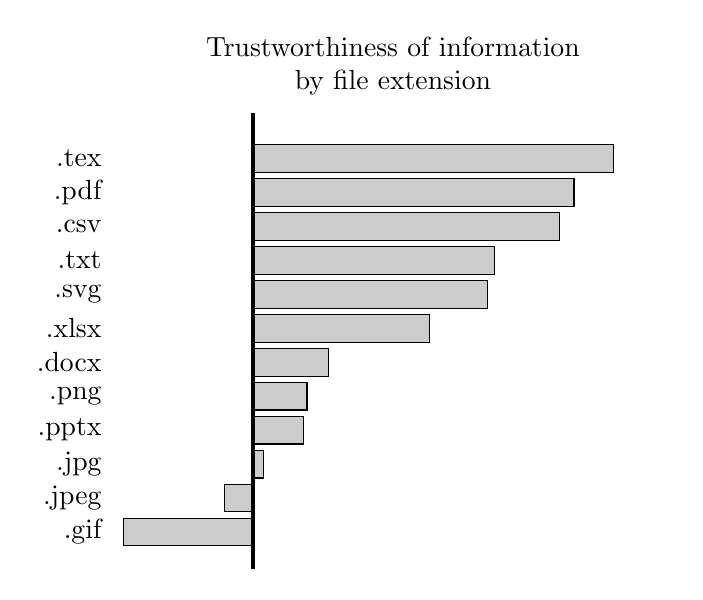
\begin{tikzpicture}


 
\begin{axis} [
    xbar,
    axis line style={draw=none},
    tick style={draw=none},
    xticklabel style={draw=none},
    % try min ticks = 12,
    ytick = {0,1,2,3,4,5,6,7,8,9,10,11},
    xmajorticks = false,
    xmin = -36,
    yticklabels={
        .gif,
        .jpeg,
        .jpg,
        .pptx,
        .png,
        .docx,
        .xlsx,
        .svg,
        .txt,
        .csv,
        .pdf,
        .tex
    },
    % title style={align=left},
    title style={text width=6cm},
    title = {\centering Trustworthiness of information\\by file extension\\},
    ]
\addplot [
    fill = black!20!white,
    draw = {black},
    % style = {thick},
]
coordinates {
    (-36,0) 
    (-8,1) 
    (3,2) 
    (14,3)
    (15,4)
    (21,5)
    (49,6)
    (65,7)
    (67,8)
    (85,9)
    (89,10)
    (100,11)
};

\end{axis}

\draw[ultra thick] (1.65,0) -- (1.65,5.8);
 
\end{tikzpicture}
 
\end{document}
